\documentclass[10pt,twocolumn,letterpaper]{article}

\usepackage{iccv}
\usepackage{times}
\usepackage{epsfig}
\usepackage{graphicx}
\usepackage{amsmath}
\usepackage{amssymb}

% Include other packages here, before hyperref.

% If you comment hyperref and then uncomment it, you should delete
% egpaper.aux before re-running latex.  (Or just hit 'q' on the first latex
% run, let it finish, and you should be clear).
\usepackage[breaklinks=true,bookmarks=false]{hyperref}

\iccvfinalcopy % *** Uncomment this line for the final submission

\def\iccvPaperID{****} % *** Enter the ICCV Paper ID here
\def\httilde{\mbox{\tt\raisebox{-.5ex}{\symbol{126}}}}

% Pages are numbered in submission mode, and unnumbered in camera-ready
\ificcvfinal\pagestyle{empty}\fi

\begin{document}

%%%%%%%%% TITLE
\title{Detection and Recognition of Dinning Table Objects Using RGB-D Camera for Robotic Applications}

\author{Jakob Baumgartner\\
Faculty of Electrical Engineering,\\
University of Ljubljana\\
Tržaška 25, 1000 Ljubljana, Slovenia\\
{\tt\small jakob.baumgartner@student.uni-lj.si}
% For a paper whose authors are all at the same institution,
% omit the following lines up until the closing ``}''.
% Additional authors and addresses can be added with ``\and'',
% just like the second author.
% To save space, use either the email address or home page, not both
% \and
% Janez Perš\\
% Faculty of Electrical Engineering,\\
% University of Ljubljana\\
% Tržaška 25, 1000 Ljubljana, Slovenia\\
% {\tt\small janez.pers@fe.uni-lj.si}
}

\maketitle
% Remove page # from the first page of camera-ready.
\ificcvfinal\thispagestyle{empty}\fi

%%%%%%%%% ABSTRACT
\begin{abstract}
In this paper, we present a real-time method for 3D bounding box object detection and recognition in dinning tabletop scenarios using RGBD cameras, with potential applications in robotics. Our approach combines color and depth information to accurately detect and classify a variety of dinning room objects. While the accuracy of our method is not the highest among all approaches, it is able to achieve good performance in a real-time setting, making it suitable for use in robotics applications. We evaluate the performance of our method on the SUN-RGBD dataset, a widely used benchmark for 3D object recognition, and demonstrate its real-time capabilities using Intel RealSense camera. The results of our experiments show that our method is able to achieve competitive accuracy while maintaining a high frame rate, making it a promising solution for object detection and recognition in robotics.
\end{abstract}

%%%%%%%%% BODY TEXT
\section{Introduction}


RGBD (Red, Green, Blue, Depth) sensors\cite{Tychola_Tsimperidis_Papakostas_2022} use a combination of traditional RGB (Red, Green, Blue) cameras, which capture colour information about an object, and depth sensors, which measure the distance from the sensor to the object. In the context of a dining table, RGBD sensors can be used to allow the robot to recognise and classify a variety of objects, including dishes, glasses, utensils and food items. By combining the colour information from the RGB cameras with the depth information from the depth sensors, the robot is able to create a detailed 3D model of the objects on the table, allowing it to understand their shape, size and orientation. 

RGBD object detection and classification algorithms have a number of advantages over traditional object detection algorithms that rely solely on colour information\cite{Rosin_Lai_Shao_Liu_2019}. One advantage of using RGBD information is that the algorithm can better handle occlusion and clutter in the scene. Occlusion occurs when an object blocks the view of another object, and clutter refers to the presence of multiple objects in the scene that may be difficult to distinguish. By using depth information, the algorithm can better understand the spatial relationships between objects and more accurately detect and classify objects even when they are partially occluded or surrounded by clutter. Example of occlusion on a dining table is when a plate is partially hidden behind a glass. Another benefit of using RGBD information is that it enables the algorithm to better distinguish between objects that are similar in colour but different in shape or size. This can be particularly useful when there are multiple objects of the same colour in the scene, as the algorithm can use the depth information to distinguish them based on their shape and size. In our case it can help us distinguish between colourful tablecloths as a background and objects sitting on them. 

However, using RGBD object detection is still less common than using RGB object detection. One reason is that RGB sensors are more common and less expensive than RGBD sensors. As a result, there are more and better quality RGB than RGBD data sets. This has partially changed with the appearance of commercial sensors such as Microsoft Kinect and Intel Real-Sense. In addition, algorithms using RGBD data often require more computing power and resources to analyse the data, which can complicate implementation in real-time applications or on resource-constrained devices. In addition, RGBD data can be noisy and inaccurate, especially in low light or at long distances, which can affect the performance of the object detection algorithm. This can make it difficult to achieve the same level of accuracy and robustness as with the RGB object detection algorithms. This can be partially corrected with indoor artificial light, but is difficult under natural conditions.

We developed an algorithm that uses an RGBD sensor to detect bounding boxes around objects sitting on a dining table in real time. The algorithm also classifies the objects within these bounding boxes and accurately identifies the type of each object. This system is designed to work effectively in a dynamic environment, such as a dining room, where items may be frequently added to or removed from the table. The ultimate goal of this project is to develop a system that can assist in tasks such as identifying and organising objects on the dining table, or providing a user with information about the table's contents.
%-------------------------------------------------------------------------

\section{Related Work}

There are a number of approaches to RGB object detection, including traditional computer vision techniques and machine learning-based approaches. CNNs are particularly effective in image recognition tasks and are widely used for object recognition in a variety of fields, including computer vision, image processing, and autonomous systems. Because of the smaller data dimension, algorithms using RGB data generally run faster than algorithms using RGBD data and are widely used in robotics. Some of the networks that currently get the best results in the Coco dataset are: EVA\cite{EVA}, DyHead\cite{DYHEAD} and Focal-L\cite{Focal-L}. 

While algorithms using RGBD data are not as well developed as algorithms using RGB data, there are a number of existing algorithms\cite{Wang_Wang_Long_Gu_Li_2021}. These can be roughly divided into outdoor and indoor algorithms. This is because indoors we can use sensors that give us dense depth images, while outdoors due to lighting conditions we have to use scanners that give us sparse depth images. Another way to split detection and classification algorithms is between traditional and deep learning methods. Algorithms in both categories mostly follow the same pipeline. First we create region suggestions and then classify them. Traditional methods rely on handcrafted functions, while deep learning methods replace one or more of the algorithm parts with deep neural networks. Despite extensive research, the performance of traditional methods is still far from that of the human visual system. Traditional methods often lose performance when dealing with crowded scenes and scenes with high occlusion. Deep learning methods have solved some or most of these problems. Objects that our algorithm recognises are similar to the objects contained in the data set SUN-RGBD\cite{7298655} \cite{SUNRGBDweb}. Deep learning models with the best performance in the data set based on mAP@0.25 are DeMF\cite{DeMF}, CaGroup3D\cite{CAGroup3D} and FCAF3D\cite{FCAF3D}. However, these algorithms are computationally intensive and cannot be executed in anywhere near real-time on normal computing devices. Since one of our goals is real-time execution, algorithms that are more comparable to ours are Frostum PointNet\cite{Qi_Liu_Wu_Su_Guibas_2018}, Frostum VoxNet\cite{Shen_Stamos_2020a} and Frostum VoxNet v2\cite{Shen_Stamos_2021}. These offer slightly worse but still impressive detection while operating at 5-10Hz.

\section{Methods}


\begin{figure*}
\begin{center}
  \makebox{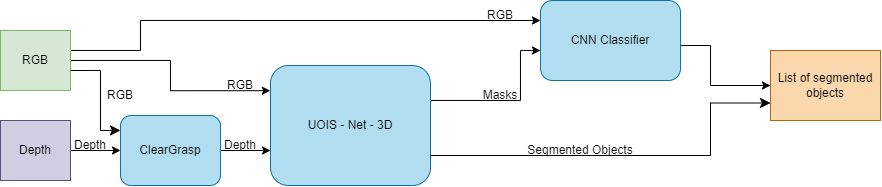
\includegraphics[width=0.75\paperwidth]{latex/structure-graph.png}}
\end{center}
   \caption{Full proposed framework pipeline.}
\label{fig:structure-graph}
\end{figure*}



% overview
Our framework consists of three separate components, as can be seen in the figure \ref{fig:structure-graph}. Together, they allow us to solve the problem of instance segmentation and classification of objects on a dinner table in a real-world environment. The input to our pipeline is a single RGBD image. Our method returns a list of segmented instances with segmentation masks and the positions of the objects. Our method also returns classifications for objects that are common in the given environment.

The first component in our framework is a depth estimator for transparent objects \cite{Sajjan_Moore_Pan_Nagaraja_Lee_Zeng_Song_2019}. Transparent objects are common elements in our application environment. One of the most common categories on dinner table are transparent glasses for sodas and juice. Transparent bottles and salad bowls are also common. Transparent objects possess unique visual properties that make it incredibly difficult for standard 3D sensors to make accurate depth estimates. They do not adhere to the geometric light part assumptions of classic stereo vision algorithms, the consequence of which is that commercially aveliable sensors producing noisy or distorted approximations of the surfaces behind them. To solve this problem, we use the ClearGrasp algorithm to derive the depth data of the transparent objects from the RGB data and the surrounding non-transparent surfaces.

The second component in our pipeline is an Unseen Object Instante Segmentator (UOIS) \cite{Xie_Xiang_Mousavian_Fox_2021}. Due to the unstructured nature of our task, it is infeasible and impractical to model every possible object in our environment. For a robot to successfully manipulate objects on a dining table, it must be able to recognise and segment instances of previously seen as well as unseen objects \cite{Xie_Xiang_Mousavian_Fox_2020}. This component takes as input RGB and point cloud data and provides segmentation masks and positions for each known and unknown object on the dining table. It is able to segment objects even if they are cluttered together or partially occluded. Before we can use this stage we need to backproject Depth image to Point-Cloud data \cite{Bostanci_Kanwal_Clark_2015}, for this we need to know the intrinsic matrix of the camera used.

The third component of our framework is a CNN classifier. UOIS provides instance segmentation masks. With these, we can cut out individual objects and then perform a classification for the common objects on a dining table. These detections can be passed on to the robot so that it can separate kitchen utensils such as plates, cups and cutlery from other objects and the rubbish left on the table.

% clearview

\subsection{Transparent objects depth estimator}

\begin{figure}
\begin{center}
     \makebox{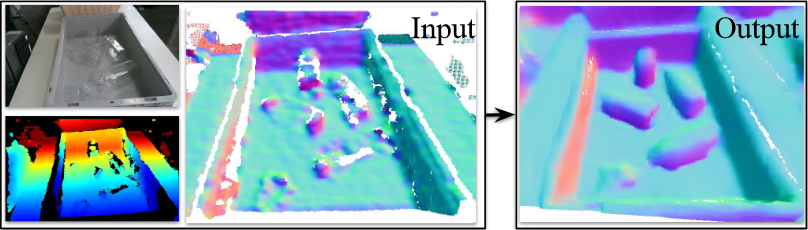
\includegraphics[width=1\linewidth]{latex/ClearGrasp.png}}
\end{center}
   \caption{We use ClearGrasp algorithm to estimate missing depth data of transparent objects.}
\label{fig:ClearGrasp}
\end{figure}

Transparent objects do not adhere to the geometric assumptions about the light path made in classical stereo vision algorithms. This makes it difficult for commercial 3D sensors to correctly detect depth information. ClearGrasp is an algorithm that leverages deep learning with synthetic training data to create accurate depth profiles of transparent objects.

\subsubsection{Method}

ClearGrasp algorithm \cite{Sajjan_Moore_Pan_Nagaraja_Lee_Zeng_Song_2019} is a modified version of completion pipeline proposed by Zhang and Funkhouser \cite{47764}. Algorithm consists of four stages.

\textbf{Transparent object segmentation}
At this stage we use an image segmentator to predict pixel-wise masks of transparent objects. For this we use Deeplabv3+ \cite{7913730} \cite{Chen_Zhu_Papandreou_Schroff_Adam_2018} with a DRN-D-54 \cite{Zhang_Funkhouser_2018} backbone to remove all depth pixels corresponding to transparent surfaces.

\textbf{Surface normal estimation}
In this stage we also use a combination of Deeplabv3+ with a DRN-D-54 backbone, this time to predict surface normals on the RGB input image.

\textbf{Boundary Detection}
In the next stage, we again use a combination of Deeplabv3+ and DRN-D-54, this time to label each pixel of the RGB image into one of three categories. The categories are Non-Edge, Occlusion Boundary (object behind another) and Contact Edges (objects sticking together).

\subsubsection{Global Optimisation for Depth}
Finally, we can use the depth image with the removed pixels of the transparent objects, the surface normal predictions, the occlusion edges and the contour edges obtained in the previous steps to reconstruct the missing depth regions of the transparent objects.
\[E = \lambda_D E_D\ + \lambda_S E_S\ + \lambda_N E_N\]
At this stage, we solve a system of equations with the aim of minimising the weighted sum of the squared errors of three terms: \(E_D\) - distance between estimated and observed depth, \(E_S\) - difference of distance between depths of neighbouring pixels and \(E_N\) - measure of difference between estimated depth and predicted surface normals. \(\lambda\) are the weights of the different terms.

An example of the prediction method is shown in \ref{fig:ClearGrasp}

\subsubsection{Dataset}

The algorithm was trained on a synthetic dataset with nearly 50,000 distinct instances. Blender's physics engine with the ray tracing rendering engine Blender Cycles was used to create the dataset. 9 different CAD models of transparent objects, many different background textures and different simulated lighting conditions were used. Each instance of the dataset contains an RGB image, a depth image, semantic segmentations of all transparent objects, the camera position, the poses of all objects and the surface normals image. 


% UOIS

\subsection{Unseen Object Instance Segmentator}

To divide cluttered objects on the dining table into individual instances, we use Unseen Object Instance Segmentator (UOIS-Net-3D) \cite{Xie_Xiang_Mousavian_Fox_2021}. The algorithm takes as input a single RGBD image and outputs object instance segmentation masks for all previously seen or unseen objects. The output of the algorithm does not contain specific categories of objects, only background, table and object instance.

The algorithm consists of separately trained neural networks and multiple stages. A simple representation of the algorithm can be seen in the figure \ref{fig:UOIS-scheme}.

\begin{figure}
\begin{center}
     \makebox{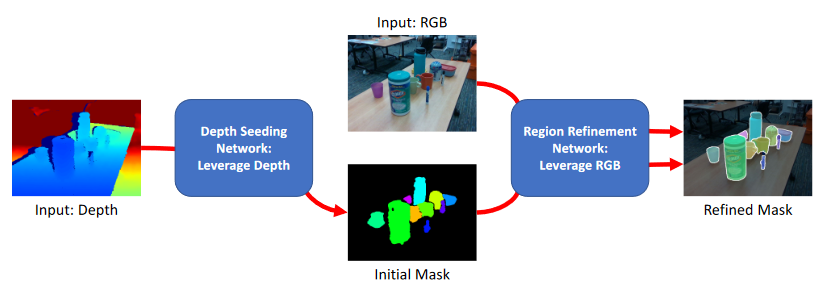
\includegraphics[width=1\linewidth]{latex/UOIS-scheme.png}}
\end{center}
   \caption{UOIS-Net-3D consists of two neural networks, that process Depth and RGB data seperately, to produce instance segmentation masks.}
\label{fig:UOIS-scheme}
\end{figure}

\begin{figure}
\begin{center}
     \makebox{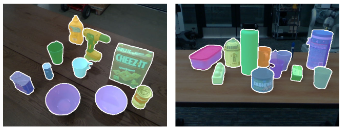
\includegraphics[width=1\linewidth]{latex/UOIS-examples.png}}
\end{center}
   \caption{We use UOIS-Net-3D algorithm to segment all objects in the image.}
\label{fig:UOIS-example}
\end{figure}

\subsubsection{Method}

\textbf{Depth Seeding Network - DSN}
The first stage of the instance segmentation network takes as input an organised point cloud D with XYZ coordinates. The reason why we use depth data first is because of the better generalisation of neural networks trained on simulated depth data to real-world scenarios, compared to networks trained on synthetic RGB data. The organised point cloud is passed through the DSN network, which returns a segmentation mask for each pixel for the given image and the 3D offsets to the object centres. \(V'\in\ \Re^{H \times W \times 3}\).

\textbf{Initial Mask Processing Module - IMP }
In this phase of the algorithm, we apply some basic image techniques to the initial segmentation mask. First, we apply an opening operation (erosion+dilation) to each mask instance to remove salt/pepper noise. Then we apply a closing operation (dilation+erosion) to remove small holes in the mask. Finally, we remove minor unconnected components of each mask. 

\textbf{Region Refinement Network - RRN}
At this stage, we use another neural network to refine the segmentation mask obtained from the depth image with additional RGB information. The input of the RRN is a 4-channel cropped image consisting of a concatenated cropped RGB and a single object mask. We use a U-Net network architecture.
During the training process, we first train the DSN network and then use the output segmentations for RRN training. During training, we first use the segmentation masks before input to the RRN. This allows us to simulate the noise and errors that occur when using data from a real depth sensor but are not seen on the clear synthetic images. For pertrubation, we use augmentation techniques such as translation, rotation, addition, cutting, morphological operations and random elipses. For an example of a segmentation result, see image \ref{fig:UOIS- example}. 

\subsubsection{Dataset}
The method was trained on a synthetic dataset called the Tabletop Object Dataset (TOD). The dataset consists of 40,000 synthetic scenes. Each scene consists of a SUNCG home environment. In this environment is a ShapeNet model of a table with 5 to 25 ShapeNet \cite{Chang_Funkhouser_Guibas_Hanrahan_Huang_Li_Savarese_Savva_Song_Su_et} models of objects randomly placed or stacked on the table. For each object, the constalation dataset contains seven different views. Due to the limitations of the simulator used (PyBullet), RGB textures do not look photorealistic. The depth data, while clear compared to data from an actual commercial sensor, is closer to a realistic representation. A synthetic dataset was used as there is no reliable tabletop data taken in the real world.

% CNN

\subsection{Classifier}
The final component of our pipeline is an image classification network. We use segmentation masks obtained from UOIS to cut out each object from the RGB image and then use the ResNet convolutional model to classify each object into one of the categories listed. The categories are: Cup, Plate, Bowl, Glass, Cutlery, Purse, Napkin, Tin, Bottle, Other. The idea behind this is that a robot working in the hospitality industry can divide the objects into a section for laundry and a section for the bin / other objects.

\textbf{Dataset}
To train our classifier, we used images from the ImageNet dataset for the specified categories. ImageNet consists of more than 20,000 categories, but we selected for training only images from the categories we chose and a set of images with random objects to train the so-called "other" category. Half of the images we selected are from objects we want to classify and the other half of the images are from a number of different uncategorised objects.

% Hardware

\section{Experiments}
In order for our framework to be useful for robotic applications, it must be able to work with a high success rate in each part of the pipeline and execute at a reasonable speed. In the experimental part of this article, we therefore focus on testing parts of the pipeline individually and in conjunction with others.

To perform the experiments, we have created the pipeline of algorithms described. We use PyTorch \cite{Paszke_Gross_Massa_Lerer_Bradbury_Chanan_Killeen_Lin_Gimelshein_Antiga_et} implementations of each of the methods described above. To avoid problems with different versions of PyTorch as well as other dependencies, we run each of the components in a separate Docker container.

The experiments were conducted on a computer with Intel® Core™ i7-12700 CPU,
GEFORCE GTX 1080 Ti GPU and 32GB of RAM performed.

\subsection{Object Segmentation Database (OSD)}

Our experiments can be divided into two parts. First, we tested our system with the Object Segmentation Database (OSD).

We perform an ablation experiment to see how removing the augmentation network for transparent objects at the beginning of the pipeline affects the segmentation and classification results. The purpose of this test was to see if using augmented data affects the segmentation of non-transparent objects in any way.

We test how accurate our classifier is.

We also measure the time it takes each of the pipeline components to perform computations. We pay attention to how the number of opaque objects affects the computation times.

\subsection{Intel RealSense D435}

In the second part of the experiments we use the Intel RealSense D435 camera to capture a series of RGBD images. The goal of this experiment is to see if our pipeline works on new data. Besides general examples, we use the camera to capture several RGBD images of situations that are not included in the OSD database.

We take 25 different images that contain transparent objects. We then compare the results of segmenting transparent objects with and without using the ClearGrip component to enhance the depth images.

Then we take a series of images of small and thin objects. The RGBD camera has a resolution of 2\% error at distances of less than 1m. This means that certain small or thin objects are not visible on the depth image. Examples of such objects are cutlery, paper pages or menus. We want to test whether the segmentation algorithm used can recognise these objects based on RGB data alone. Since the first detection step in the UOIS uses depth information, we expect that these objects will not be detected.


% with/without ClearGrip

% UOIS-3D-Net

% MaskRCNN - can I train this?!? dataset err

% Klasifier

% Time

% Dataset






{\small
\bibliographystyle{ieee_fullname}
\bibliography{egbib}
}

\end{document}
